\documentclass{sig-alternate-ipsn12}

%\usepackage{url}
%\usepackage{cite}
%\usepackage{graphics}
%\usepackage{graphicx}
%\usepackage{epsfig}
%\usepackage{amssymb}
%\usepackage{amsthm}
%\usepackage{lineno}

\hyphenation{op-tical net-works semi-conduc-tor}

\begin{document}
\title{Performance Evaluation of Routing Protocols for Mobile Wireless Sensor Networks}

%\author

\maketitle

\begin{abstract}
In \emph{Wireless Sensor Networks} (WSNs), node mobility can increase the network capability in many aspects, such as automatic node deployment, flexible topology adjustment, and rapid event reaction.
Nevertheless, most of the routing protocols for WSNs are mainly designed for static networks, especially in IEEE 802.15.4 standard which its support for mobile networks is yet to be established.
This paper evaluates several routing protocols for ad hoc networks in a WSN environment in order to investigate how such protocols perform in terms of data delivery ratio and routing overhead.
We also present \emph{Ant-based Dynamic Hop Optimization Protocol} (ADHOP), a self-configuring reactive routing protocol for mobile WSNs.
ADHOP is based on \emph{Ant Colony Optimization} (ACO) which allows us to deal with the restrictions of WSNs and yet improve the route discovery and the route maintenance through pheromone.
Our routing algorithm has been evaluated, validated, and compared to other well-known protocols through a IEEE 802.15.4 network.
We have obtained better results in terms of data delivery ratio, routing overhead, and congestion avoidance for environments of dynamic topology.
\end{abstract}

%\IEEEpeerreviewmaketitle

\section{Introduction}
\label{introduction}

WSN consists of a set of spatially distributed sensor nodes which monitor structures, machinery, and environmental conditions.
Sensor nodes are characterized by their constraints in processing power, memory, bandwidth, and energy consumption \cite{Matrouk:2009}.
They are often deployed in harsh environments.
As a result, node damage and failure become common events.
Therefore, associated routing protocols must dynamically handle network topology changes.
This adds to the typical topology change of \emph{Mobile Ad Hoc Networks} (MANETs) due to node mobility \cite{Garcia:2007}.
Moreover, by introducing mobility to WSNs, the network capability can be improved in many aspects, such as automatic node deployment, flexible topology adjustment, and rapid event reaction \cite{Wang:2010}.
This way, routing algorithms for WSNs which handle the overhead of topology changes and mobility have attracted a significant interest \cite{Akkaya:2005, Watteyne:2010}.

Routing protocols for MANETs are usually classified in three groups: proactive, reactive, and hybrid.
Differently, routing protocols for WSNs are defined according to its applications or goals in the network.
The main challenges of routing in WSNs are to support data communication while trying to prolong the lifetime of nodes' batteries, preventing connectivity degradation, decreasing congestion, and improving energy efficiency.

In many address-based routing protocols, such as most of the routing protocols for MANETs, there is a lack of global identification along with random deployment of sensor nodes which makes it hard to select a specific set of nodes to be queried \cite{Akkaya:2005}.
Therefore, data-centric routing protocols which are able to select a set of sensor nodes during the relaying of data have been considered to reduce the transmitted redundant data.
However, differently from our proposal, most of these protocols do not consider dynamic network topologies.
Hence, for contemplating the use of real WSNs with continuous changes in network topology, the construction of a protocol that handles mobility without additional overhead may have to be the first course of action.

Many routing techniques attempt to obtain reliable links among sensor nodes, since WSNs are noisy and error-prone.
Therefore, several solutions monitor the quality of links using metrics such as signal strength, data reception ratio, location, and heuristics in order to maintain reliable routes between nodes \cite{Stankovic:2008}.
Routing algorithms inspired by ant collective intelligence can be an effective way to deal with dynamic topologies.
Because of the ability of ants to perceive changes in networks by pheromone.
They usually provide the ability to learn the shortest routes \cite{Lu:2004} and yet automatically adapt to network topology changes \cite{Iyengar:2007}.
As a result, ant-based routing algorithms have been considered as an alternative for many scalable multi-hop networks \cite{Wang:2009}, including WSNs \cite{Okdem:2009, Dhurandher:2009}.

This paper evaluates several routing protocols for ad hoc networks in a WSN environment in order to investigate how such protocols perform in terms of data delivery ratio and routing overhead.
We also propose ADHOP, a self-configuring and multi-hop reactive routing protocol which aims at providing a low-overhead routing for mobile WSNs.
It allows us to deal with the overhead of dynamic topologies taking into account congestion and unreliable routes between nodes.
ADHOP uses a dynamic hop method to improve the routing decisions in mobile WSNs.
Our approach uses the ant collective behavior to make routing decisions by pheromone and some heuristic information.
By using pheromone, ADHOP is able to adapt to network changes, such as mobility and node failures.
ADHOP was designed to use one or more heuristic information to support routing decisions according to the network needs, such as distance, latency, residual energy, and \emph{Received Signal Strength Indicator} (RSSI).
These contributions allow us to achieve a routing algorithm powerful enough to ensure reliable routes among nodes and yet handle congestion in dynamic topology environments.

% + Paper organization
The remainder of this paper is organized as follows: section \ref{related_work} presents related work.
In section \ref{proposed}, we explain and describe ADHOP.
In section \ref{evaluation}, we analyze and evaluate several routing protocols for MANETs in an IEEE 802.15.4 network.
We also explain about our implementation by evaluating and comparing ADHOP with such protocols.
Finally, we present our conclusion of the study in the last section.


\section{Related Work}
\label{related_work}

% + Proactive
Proactive routing protocols usually have low latency; therefore, nodes can quickly get routes to any other node in the network.
The routes are calculated before one is needed by trying to keep the routing information to all nodes up-to-date.
As a result, all nodes need to regularly broadcast information.
\emph{Optimized Link State Routing} Protocol (OLSR) is a proactive link state routing protocol optimized for wireless ad hoc networks \cite{Clausen:2003}.
OLSR protocol sends topology control messages intermittently to discover and then disseminate link state information throughout the network.
Therefore, each node uses this topology information to compute next hop for all nodes in the network.
\emph{Destination-Sequenced Distance-Vector} (DSDV) is also a proactive routing protocol which guarantees loop-free routes \cite{Perkins:1994}.
DSDV models cooperative nodes that periodically announces the interconnection topology among nodes to provide convenient connectivity for mobile nodes in ad hoc networks.
Nevertheless, in mobile networks, due to constant changes in topology, proactive routing algorithms is not feasible.
The cost to maintain updated routes among all nodes is still very high.

% + Reactive
Reactive routing protocols does not maintain record of routes thus making the network more lightweight.
Nonetheless, the route discovery tends to cause delays in the data transmission.
It builds routes between nodes only as desired by source nodes.
\emph{Ad hoc On Demand Distance Vector} (AODV) is a reactive routing protocol designed for MANETs \cite{Perkins:1999}.
It define routes using a route request and route reply query cycle.
\emph{Route Requests} (RQ), Route Replies (RP), and Route Errors (RE) are message types defined by AODV.
Considering a high mobility and a high rate of data loss, AODV may increase the load of control packets.
Each time a route breaks, AODV flood the network with these messages to notify and/or define a new route.
Differently from our proposal, it causes overhead by clogging up the network with route requests and route repairs.
\emph{Dynamic On-demand MANET routing protocol} (DYMO) is also a reactive routing for MANET \cite{Chakeres:2009}.
It is similar to AODV, but it uses the most basic route discovery and maintenance procedures.
However, DYMO presents the same overhead of AODV in respect to highly dynamic topologies.

% + Hybrid
Hybrid routing protocols combine proactive and reactive routing schemes.
HOPNET is a multi-hop hybrid routing algorithm proposed by Thulasiram and others \cite{Wang:2009}.
It has features extracted from ZRP and involves ACO to solve routing problems.
Haas \cite{Haas:1997} proposed ZRP, a hybrid routing protocol which aims to reduce the control overhead of proactive protocols and the latency of reactive protocols.
Each node maintains a proactive routing within its zone in order to obtain reliable link information among its neighbors.
However, differently from ZRP, HOPNET involves ant collective intelligence \cite{Dorigo:2005, Dorigo:2006} in the proactive routing in order to maintain and improve the existing routes or explore better options.
HOPNET has obtained good results in MANET environments of high scalability and high mobility.
Because of its efficiency in dealing with dynamic topology networks, our approach is inspired by many features of the HOPNET algorithm.


\section{ADHOP: \newline The Proposed Routing Strategy}
\label{proposed}

ADHOP is a self-configuring and multi-hop reactive routing protocol that aims at providing routing for mobile WSNs.
Our approach is a routing protocol which uses pheromone as a metric to make routing decisions, and uses heuristic information for pheromone deposit and evaporation ratio.
ADHOP aims at obtaining:

\begin{itemize}
\item
simple routing table structure;
\item
simple operations to handle the routing table;
\item
efficient reactive routing by pheromone;
\item
ants specialized in distributing and detecting pheromone throughout the network efficiently;
\item
low overhead for discovering and maintaining routes in WSNs.
\end{itemize}

Our algorithm is classified as a reactive routing protocol which aims at minimizing the routing overhead without compromising the data delivery ratio.
With the robustness of ACO-based protocols, it also handles important problems in ad hoc networks and dynamic network topologies by avoiding congestion, broken routes, and improving the discovery and maintenance of routes.
Meanwhile, through dynamic hops, ADHOP handles the known constraints of WSNs, such as processing power, memory, bandwidth, and energy consumption.

In most of the routing protocols, the routes to particular nodes are entirely maintained and stored in the routing tables, as exemplified in Figure \ref{moving_1}.
Furthermore, control packets have to carry the sequence of traversed nodes in order to update their routing tables.
If the target node is not stored as a destination in the source node, but it is part of any other route, then each route has to be verified minutely in order to find the destination.
The source node could also start a new search process in order to discover a new route to the external node.
Anyway, both processes can waste memory, processing and/or bandwidth.

\begin{figure}[htbp]
\centering
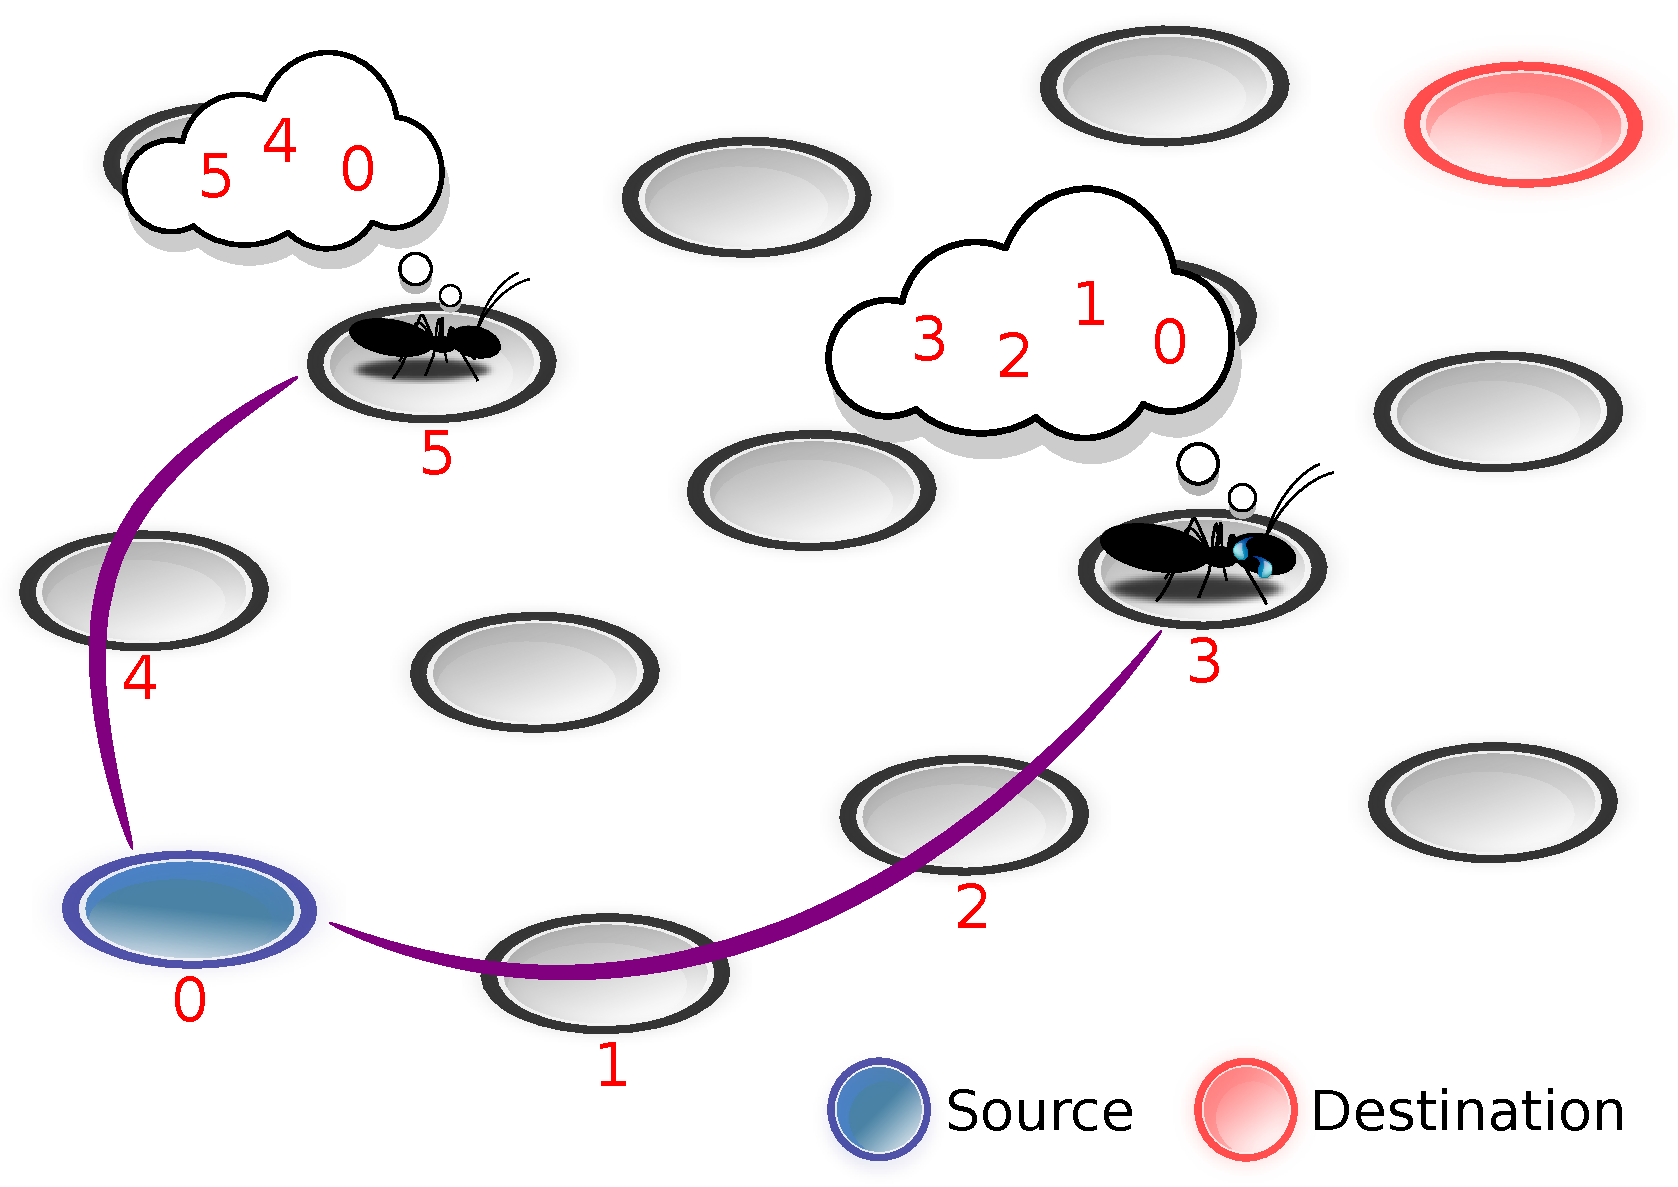
\includegraphics[width=220pt]{fig/ant_moving-1.pdf}
\caption{Routes - Sequence of Traversed Nodes}
\label{moving_1}
\end{figure}

Differently, our approach focus only on the next hop that the ant has to perform, as shown in Figure \ref{hops}.
Therefore, each node in ADHOP can store an amount of pheromone between itself and any other node in the network, i.e., all routing decisions are made locally, without needing to know the entire network to route the data.

\begin{figure}[htbp]
\centering
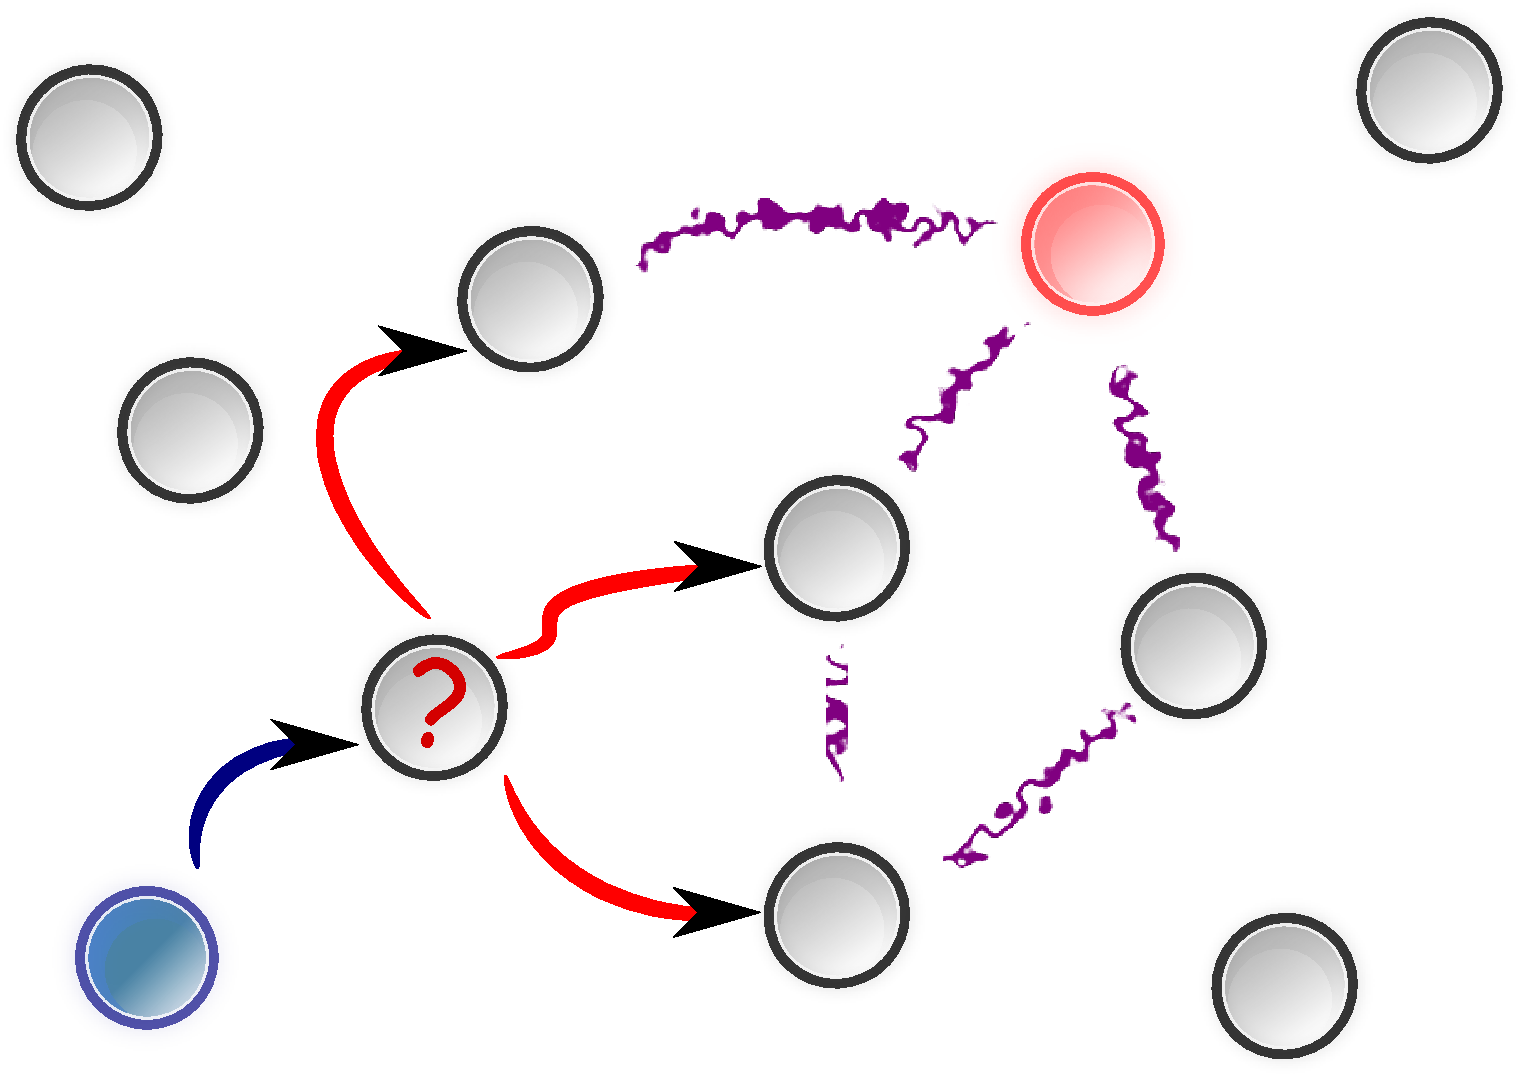
\includegraphics[width=220pt]{fig/hops.pdf}
\caption{Dynamic hops}
\label{hops}
\end{figure}

In order to make routing decisions properly, the ADHOP ants are responsible for dissipating the knowledge of the network and teaching to nodes the best route to be taken at that instant.
When an ant crosses through a node, it deposits pheromone between the neighbor node which has just crossed and the origin node, as exemplified in Figure \ref{moving_2}.
Therefore, on the way back the nodes do not need to be concerned to discover and maintain entire routes to particular nodes.
They just need to direct the ant to the next hop toward the destination node through a local decision.

\begin{figure}[htbp]
\centering
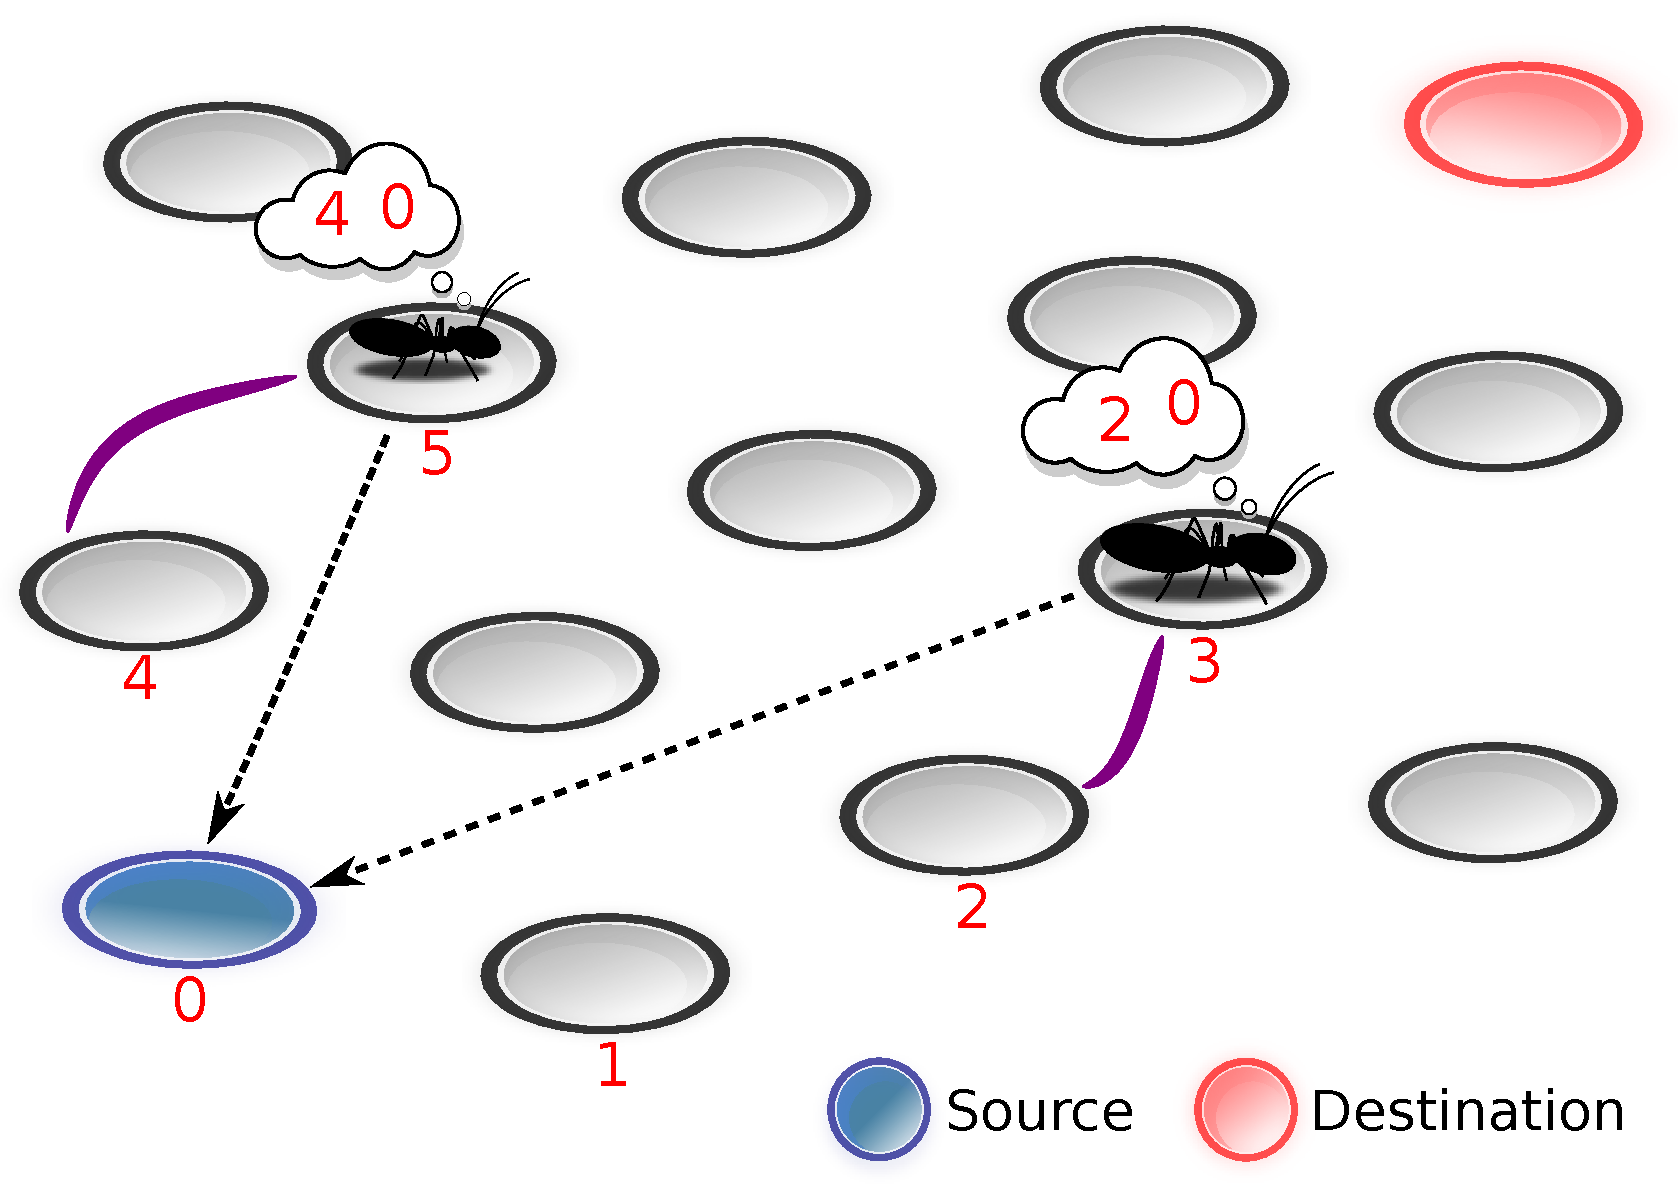
\includegraphics[width=220pt]{fig/ant_moving-2.pdf}
\caption{Routes - Dynamic Hops}
\label{moving_2}
\end{figure}

In the real world, ants communicate with each other using pheromone.
Each one takes a random walk from its anthill to search for some kind of food, as shown in Figure \ref{depositing}.
On the way back to the anthill, they deposit pheromone on the track to allow other ants to find the leftover food, reinforcing the pheromone on the trail consequently.

\begin{figure}[htbp]
\centering
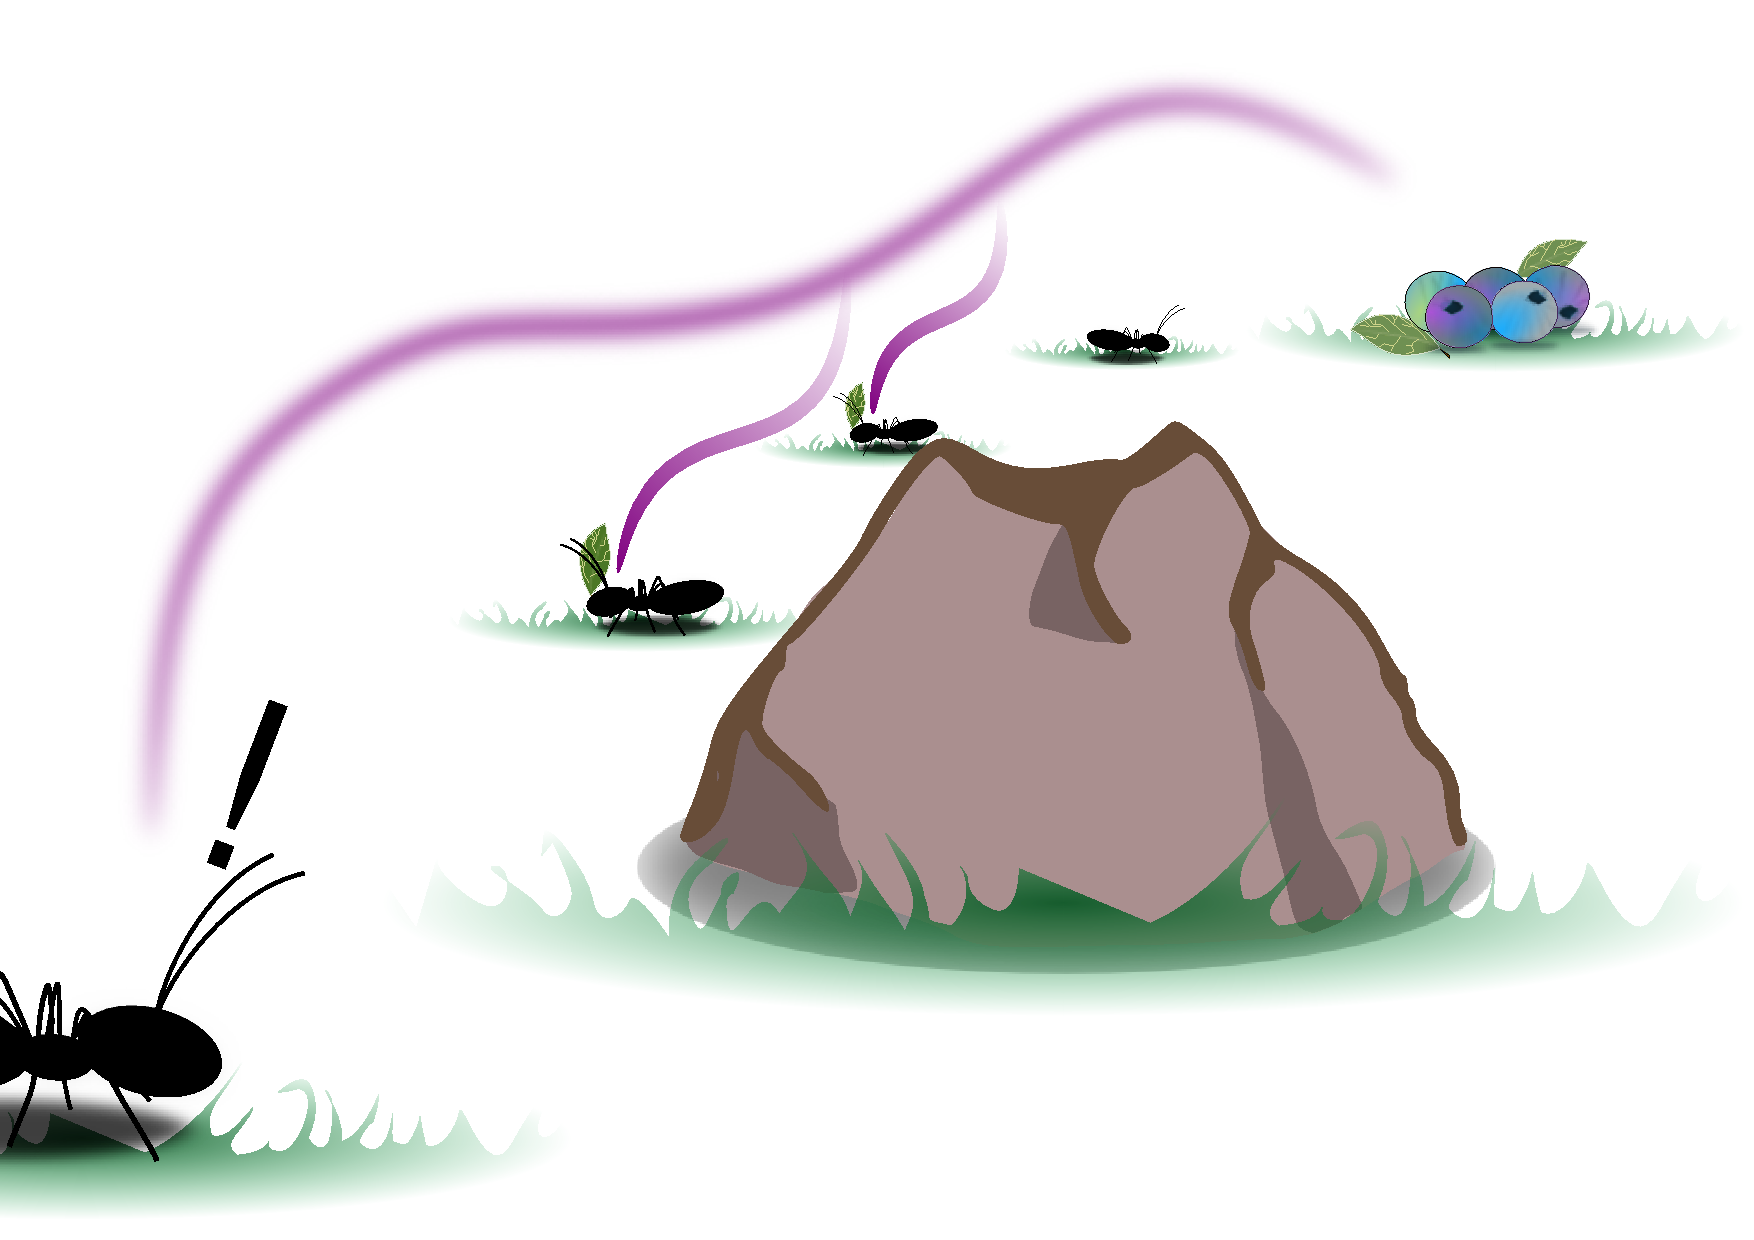
\includegraphics[width=220pt]{fig/ant_pheromone-1.pdf}
\caption{Depositing pheromone}
\label{depositing}
\end{figure}

Ants indiscriminately follow many different ways, but the pheromone reinforcement in shorter tracks tends to be more attractive.
They thereby choose the trail with the greatest pheromone amount, as shown in Figure \ref{choosing}.
However, over the course of time, the pheromone on the trail will gradually evaporate.
As a result, when the food runs out, new trails are not marked by returning ants and the pheromone slowly dissipates.
This behaviour helps ants to deal with changes in their environment.

\begin{figure}[htbp]
\centering
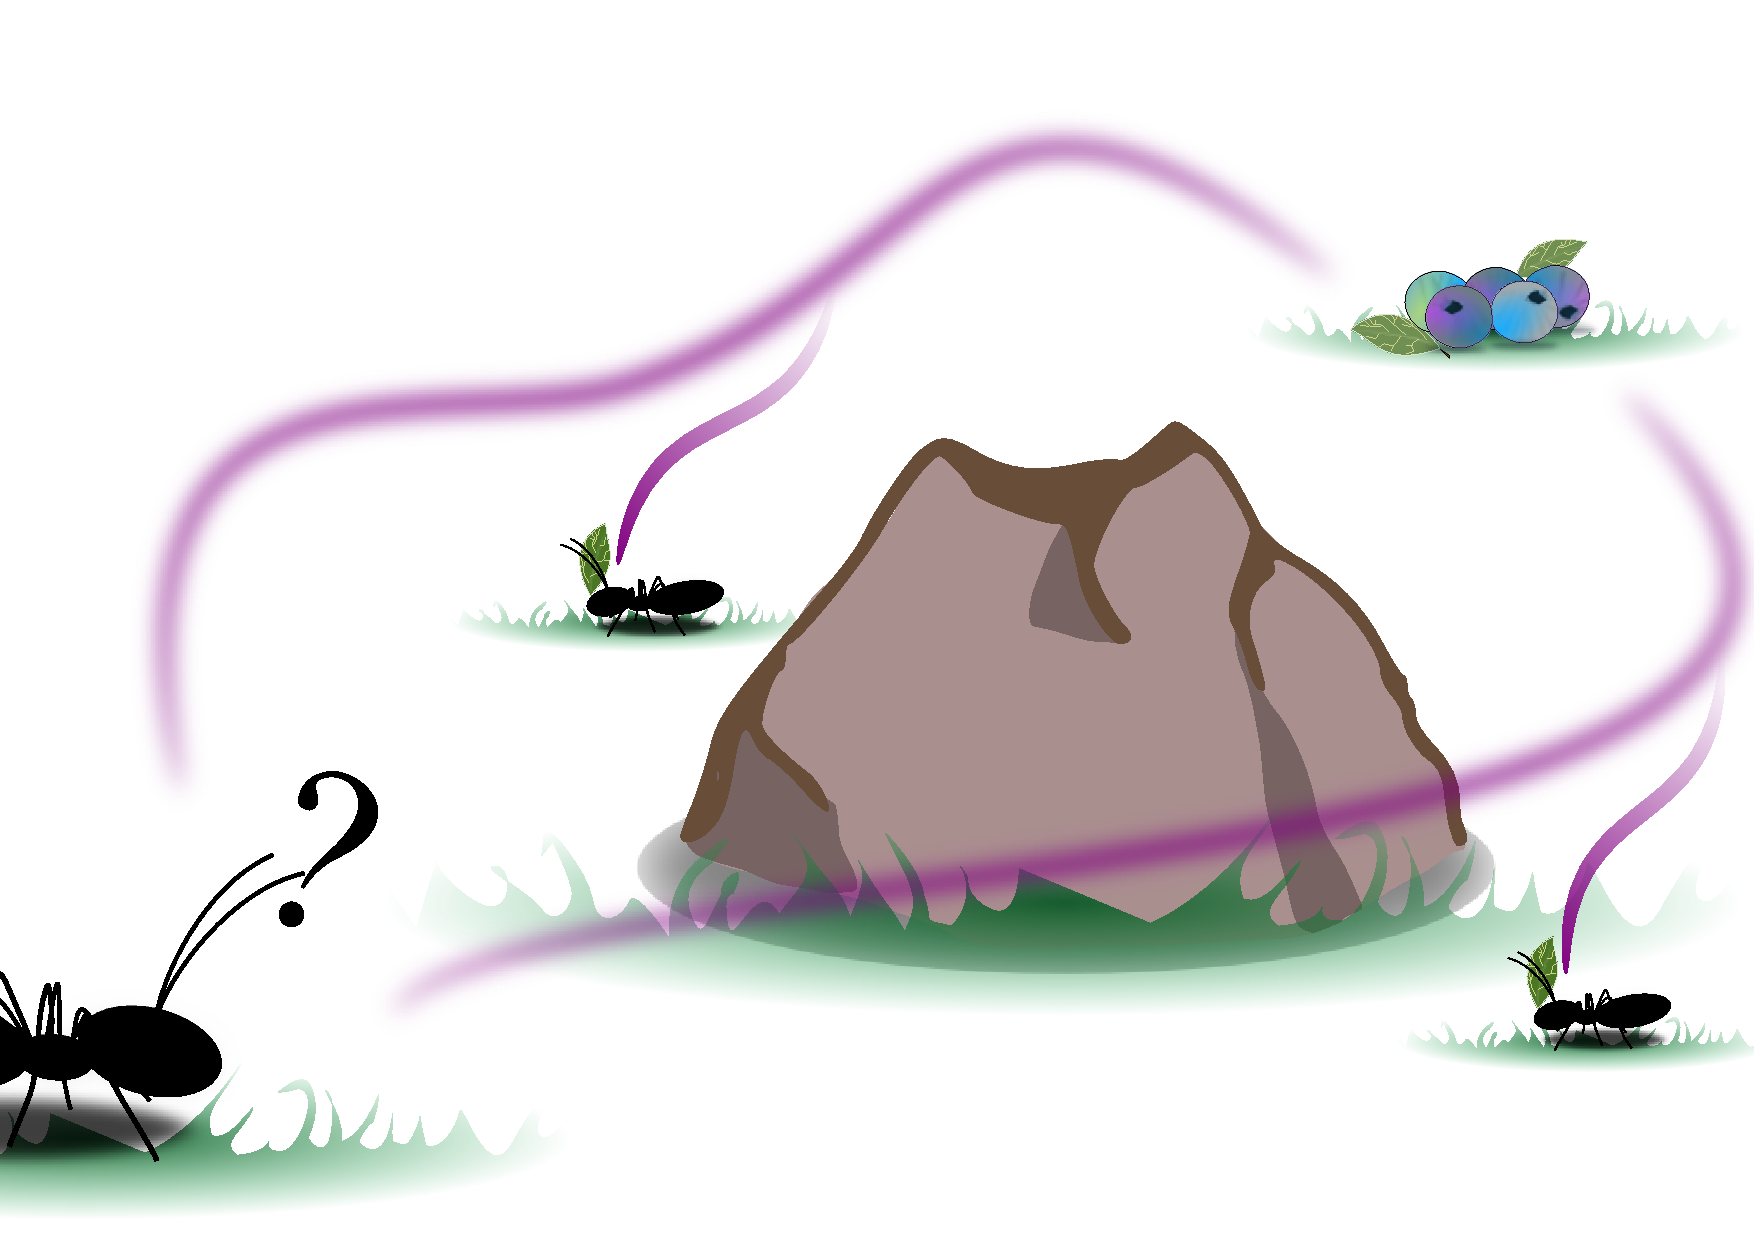
\includegraphics[width=220pt]{fig/ant_pheromone-2.pdf}
\caption{Choosing a path}
\label{choosing}
\end{figure}

The idea behind routing protocols based on ACO is to apply it to discover and maintain the best routes among nodes.
These protocols can thereby maintain the routing table updated efficiently due to the proportionate dynamism of ants to detect, by pheromone, changes in the network topology.

The ADHOP algorithm defines routes by pheromone, from the source to a particular destination.
In mobile sensor networks, nodes may fail or move away from their routes.
As a result, if a part of the route is no longer used then the other nodes eventually leaves the route due to pheromone evaporation.
In ADHOP, the routes are not predetermined and the hops are chosen dynamically at each node toward the destination (Figure \ref{hops}).
Hence, our approach adapts to topology changes and network needs transparently, as shown in Figure \ref{back_2}.

\begin{figure}[htbp]
\centering
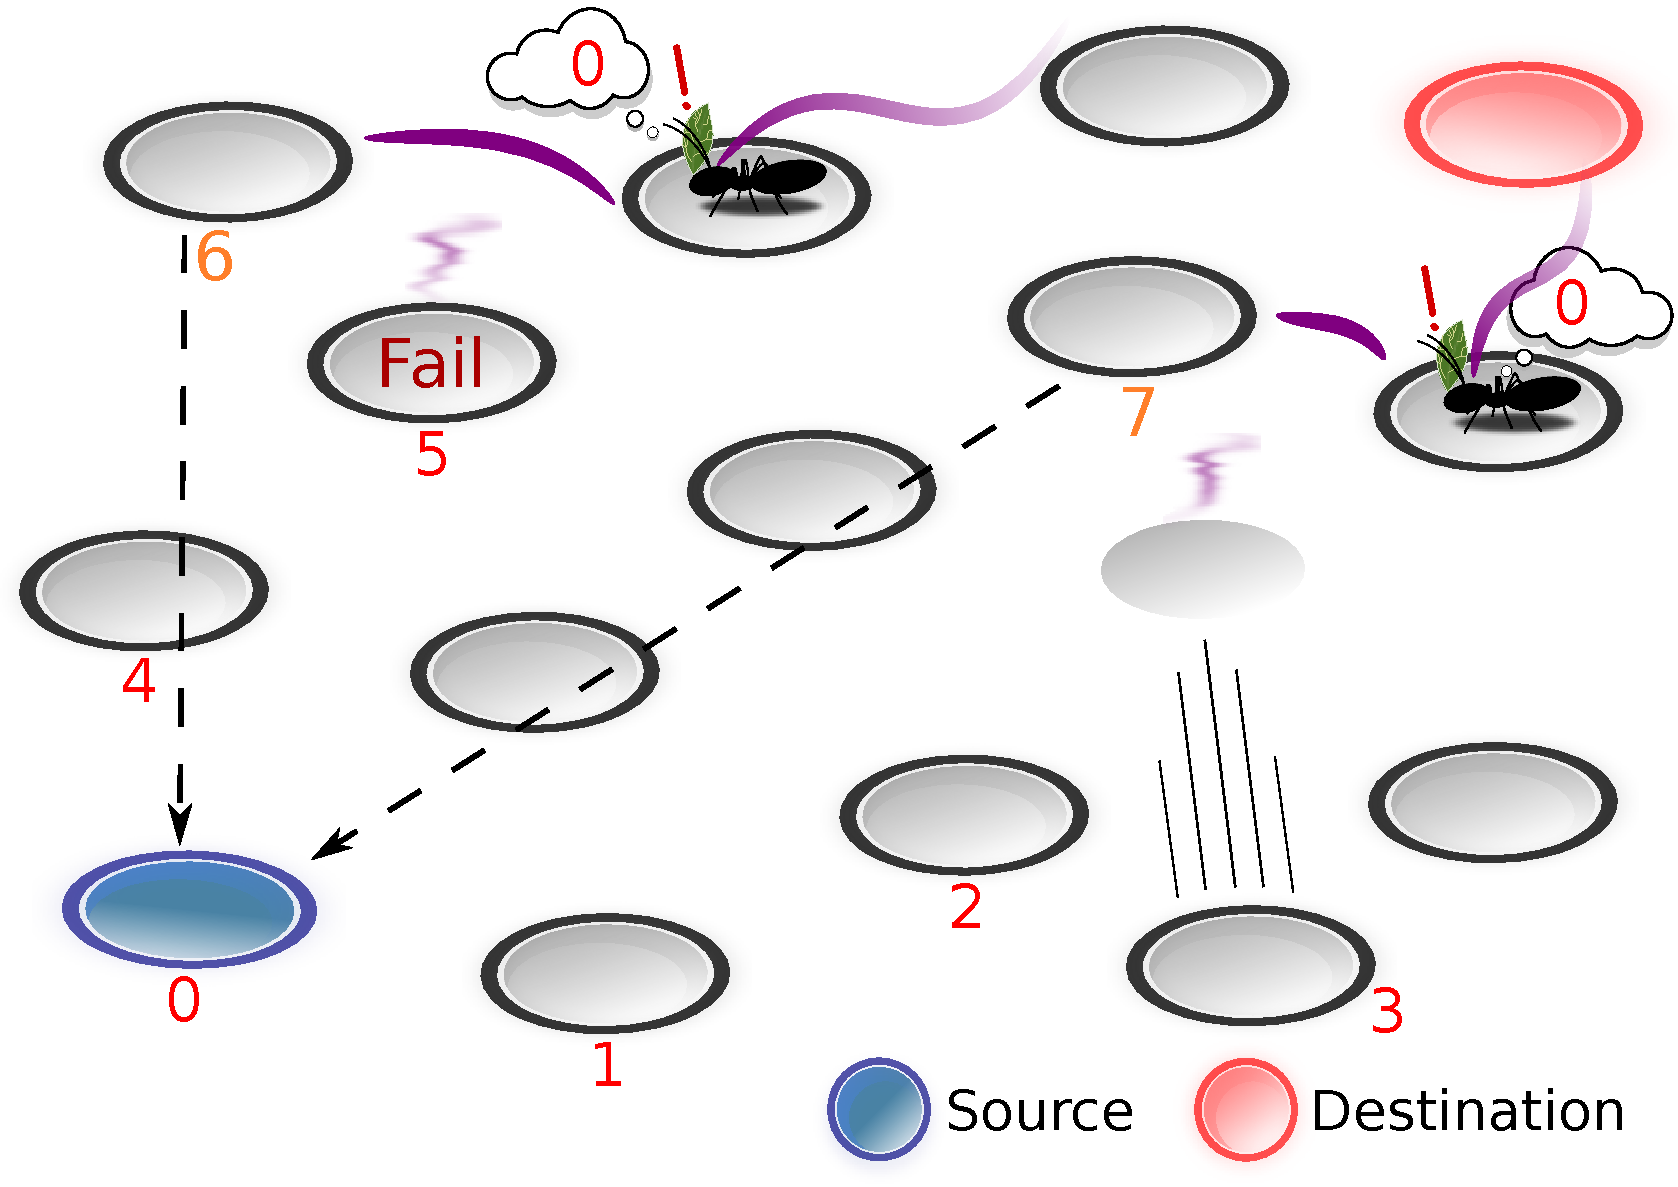
\includegraphics[width=220pt]{fig/ant_back-2.pdf}
\caption{Failed nodes and mobility, choosing an alternative path}
\label{back_2}
\end{figure}

In ADHOP, all ants map and perform the pheromone deposit, and they are responsible for maintaining the routing tables updated.
The ants use the pheromone information in order to discover and to maintain good routes.
Our routing table is a table whose rows represent its neighbors and the columns represent all identified nodes within the network.
This structure proves to be an efficient way to deal with pheromone in networks \cite{Wang:2009, Shuang:2009}.
Its operations are simpler and faster, and routes do not need to be stored entirely.
Such feature is suited for routing decisions that are made locally.
Therefore, in order to accomplish these routing operations, a new collection of ants is introduced: \emph{forward transport ant} (FTA) and \emph{exploratory transport ant} (ETA).
ETA explores new routes while FTA uses the routes discovered by ETAs.
Although each ant category has a different function, they share a common data structure.
Figure \ref{adhop_protocol} shows the ant data structure of ADHOP.

\begin{figure}[htbp]
\centering
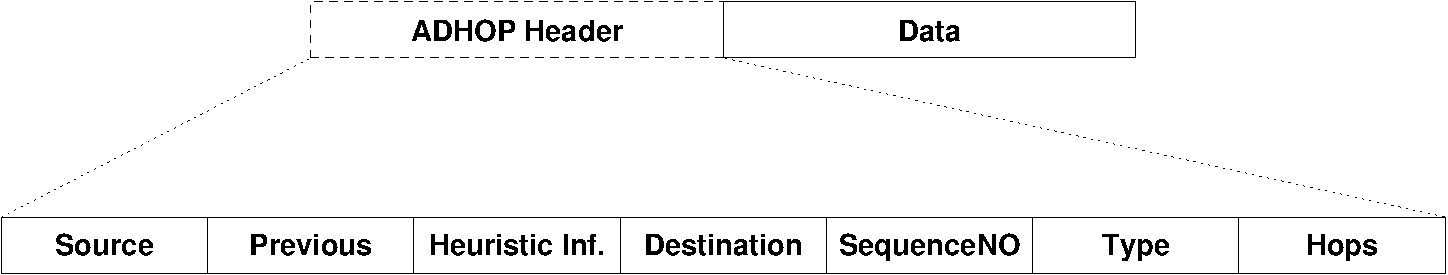
\includegraphics[width=240pt]{fig/adhop_protocol.pdf}
\caption{ADHOP Ant Structure}
\label{adhop_protocol}
\end{figure}

FTA and ETA is responsible for storing the discovered sequence of nodes into the routing table.
On the other hand, two other fields are added in order to assist with the pheromone deposit and the movements of ants among nodes.
The data structure includes address fields as \emph{Source} and \emph{Destination}.
The \emph{Previous} field is responsible for storing the address of the previous node.
The \emph{SequenceNO} field is used for control.
The \emph{Type} field indicates the ant category, and the \emph{Hops} field indicates the number of hops which the ant has done.
The \emph{Heuristic Inf.} field is responsible for storing the necessary heuristic information to calculate the evaporation and the pheromone deposit ratio.
This structure helps to reduce the complexity in offering better tactics to diffuse and verify pheromone among nodes, and to reinforce the links between neighbors to maintain the best routes as well.

In addition, both FTA and ETA perform data delivery while they deposit pheromone on the route which they travel.
This means less control packets in the network.
Such strategy is proposed considering the context of WSNs, which are noisy and error-prone.
Therefore, a routing algorithm that seeks a low overhead is the most suitable in a network of high packet loss as well as in mobile WSNs.
Hence, this study aims at efficient way to diffuse and verify pheromone in order to minimize packet loss by broken routes.

ADHOP aims at abstracting ad hoc network problems by handling topology changes only through pheromone to avoid additional overhead in the network as well as possible congestion.
Congestion usually causes packet loss, queueing delay, and consequently less pheromone deposit, especially in WSNs.
Since our routing table structure maintains pheromone information between the nodes, it does not need to be updated at each change in network topology.
These changes in topology are observed unwittingly by ants.
Thereupon, warning messages or control packets are unnecessary.
It allows us to handle congestion the way that complex operations in the network can be avoided.

We introduce the explanation of our routing scheme by means of UML sequence diagrams.
Figure \ref{adhop_data_tx} depicts the sequence diagram for data transmission in ADHOP.
The data packet is sent along with the ant to ensure that sudden changes in the network do not interfere with the transportation of the data towards the destination.
The data packet may thereby be dynamically redirected to a safer route.

\begin{figure}[htbp]
\centering
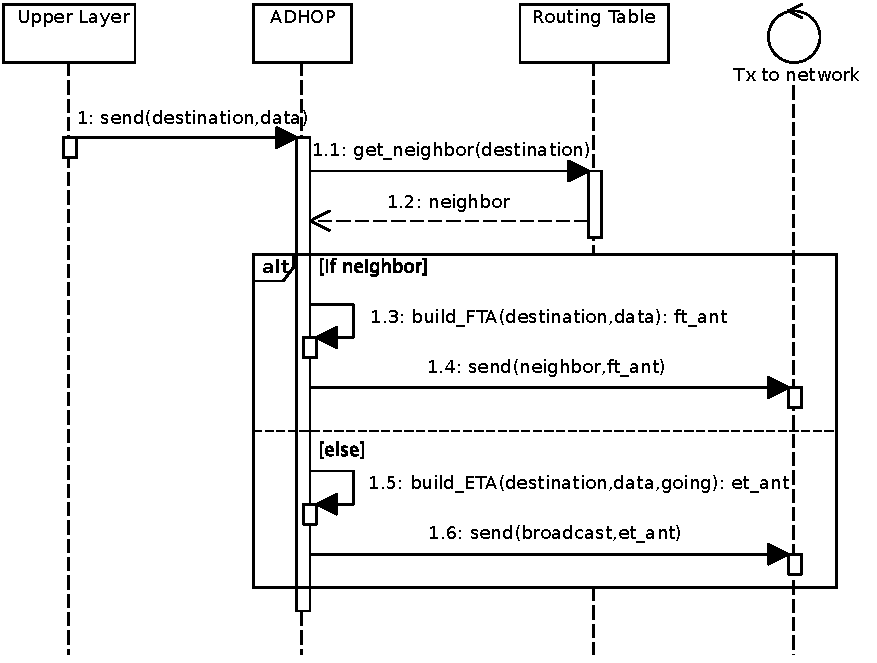
\includegraphics[width=220pt]{fig/adhop_data_tx.pdf}
\caption{ADHOP - Data Transmission}
\label{adhop_data_tx}
\end{figure}

ETAs are responsible for discovering routes to unknown nodes.
These ants travel through the network to discover the destination node.
At the destination, the ETA delivers the data packet and returns to the source node.
On the way back, the ant just sets the pheromone trail in order to reinforce the pheromone trail, as shown in Figure \ref{adhop_rx_eta}.

\begin{figure}[htbp]
\centering
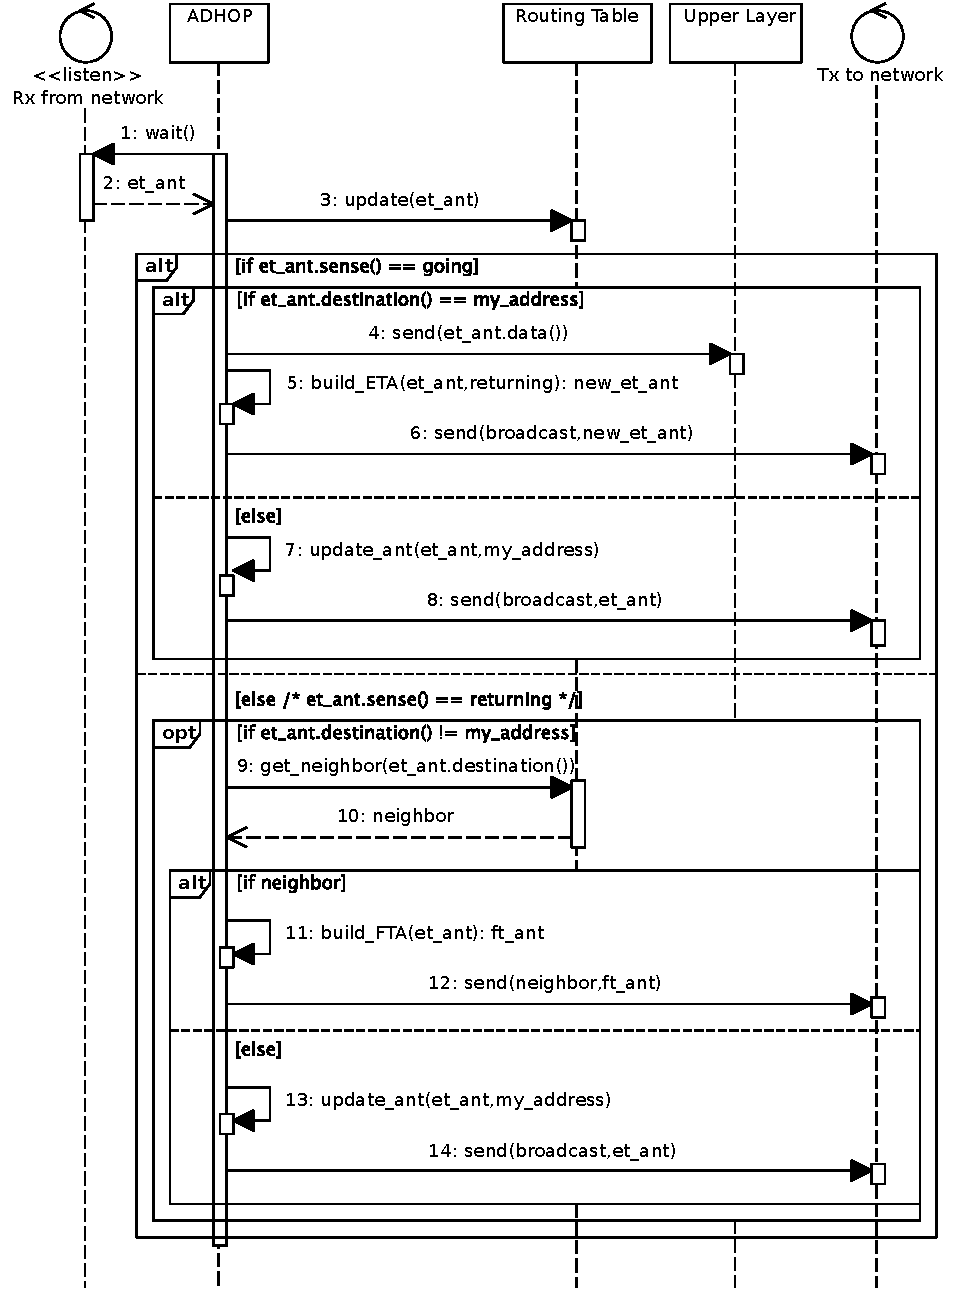
\includegraphics[width=240pt]{fig/adhop_rx_eta.pdf}
\caption{ADHOP - Rx ETA}
\label{adhop_rx_eta}
\end{figure}

FTAs are only responsible for delivering data packets to known destinations.
When a source node discovers a new route to certain destination by ETA, the following data packet transmissions are performed by FTAs until the pheromone amount on the route evaporates entirely.
Nevertheless, at any time, if any route to any destination breaks, any node on the route can use an ETA to recover it or discover a new path, as the sequence diagram shown in Figure \ref{adhop_rx_ita}.
It allows us to deal with dynamic network topologies and avoid as much as possible broken routes.

\begin{figure}[htbp]
\centering
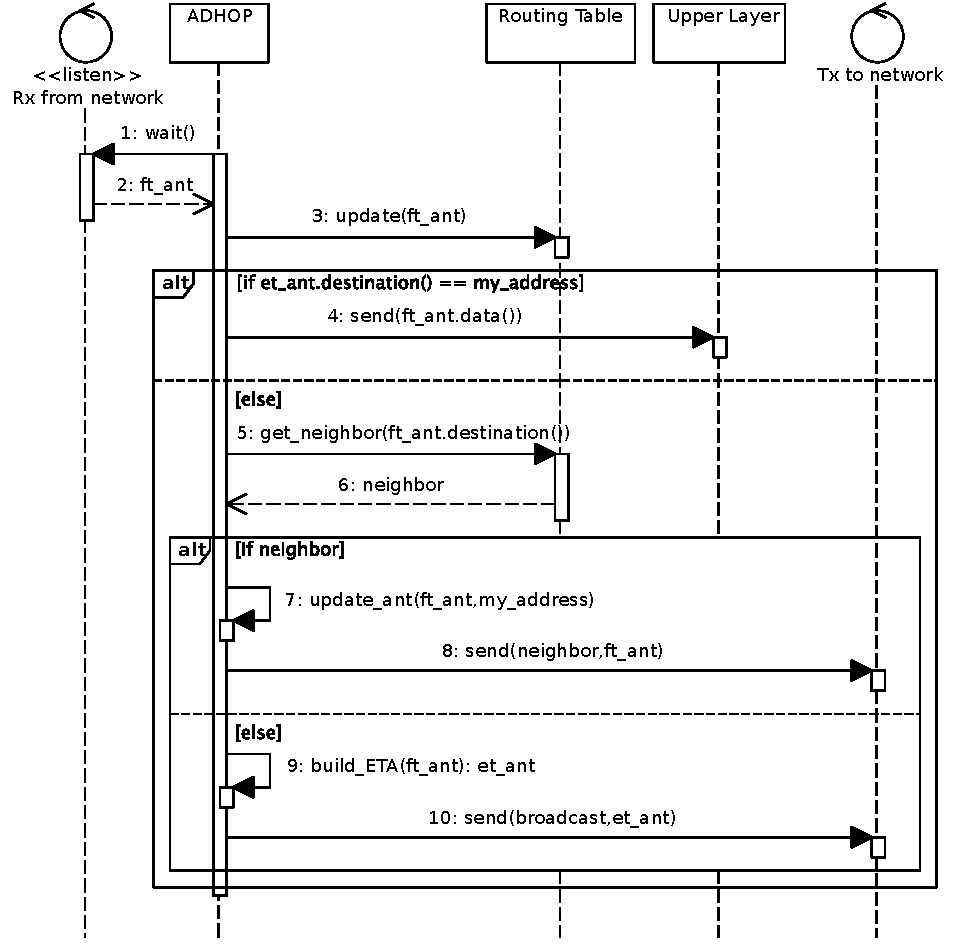
\includegraphics[width=240pt]{fig/adhop_rx_fta.pdf}
\caption{ADHOP - Rx FTA}
\label{adhop_rx_ita}
\end{figure}

Our approach uses different equations for deposit and evaporation of pheromone.
Each ant selects a node $v_{j}$ as the next hop from the current node $v_{i}$.
At the node $v_{j}$, the ant updates the pheromone $\tau _{i,s}$ on the entry $\left ( v_{i},v_{s} \right )$ in the routing table, where $v_{s}$ is the source node, as follows \cite{Dorigo:2006}:
\begin{equation} \tau _{i,s} = \left ( 1 - \varphi \right ) \cdot \tau _{i,s} + \varphi \cdot \tau _{0} \label{adhop_pheromone_increasing} \end{equation}
where $\varphi \in \left ( 0,1  \right ]$ is pheromone decay coefficient, and $\tau _{0}$ is the initial value of pheromone.
This equation allows us to diversify the search process by decreasing the pheromone amount in the routes while allowing other ants to achieve different routes.
It also helps to increase the effect of dynamic hops.

The evaporation occurs periodically to all nodes in the network, using the following equation \cite{Dorigo:2006}:
\begin{equation} \tau _{i,j} = \left ( 1 - \rho \right ) \cdot \tau _{i,j} , \quad \forall i \in N, \quad \forall j \in Z \label{adhop_evaporation} \end{equation}
where $\rho \in \left ( 0,1  \right ]$ is the evaporation rate, $N$ is the set of neighbor nodes, and $Z$ is the set of nodes which, together with neighbor nodes, define entries $\left ( v_{i},v_{j} \right )$ in routing table.

Moreover, by using Equations (\ref{adhop_pheromone_increasing}) and (\ref{adhop_evaporation}), ADHOP allows us to use several heuristics to perform the routing (e.g., as shown in Figure \ref{heuristics}).
The pheromone decay coefficient and the evaporation rate can be calculate using such information thus improving the routing in terms of which heuristic is needed for a particular application.

\begin{figure}[htbp]
\centering
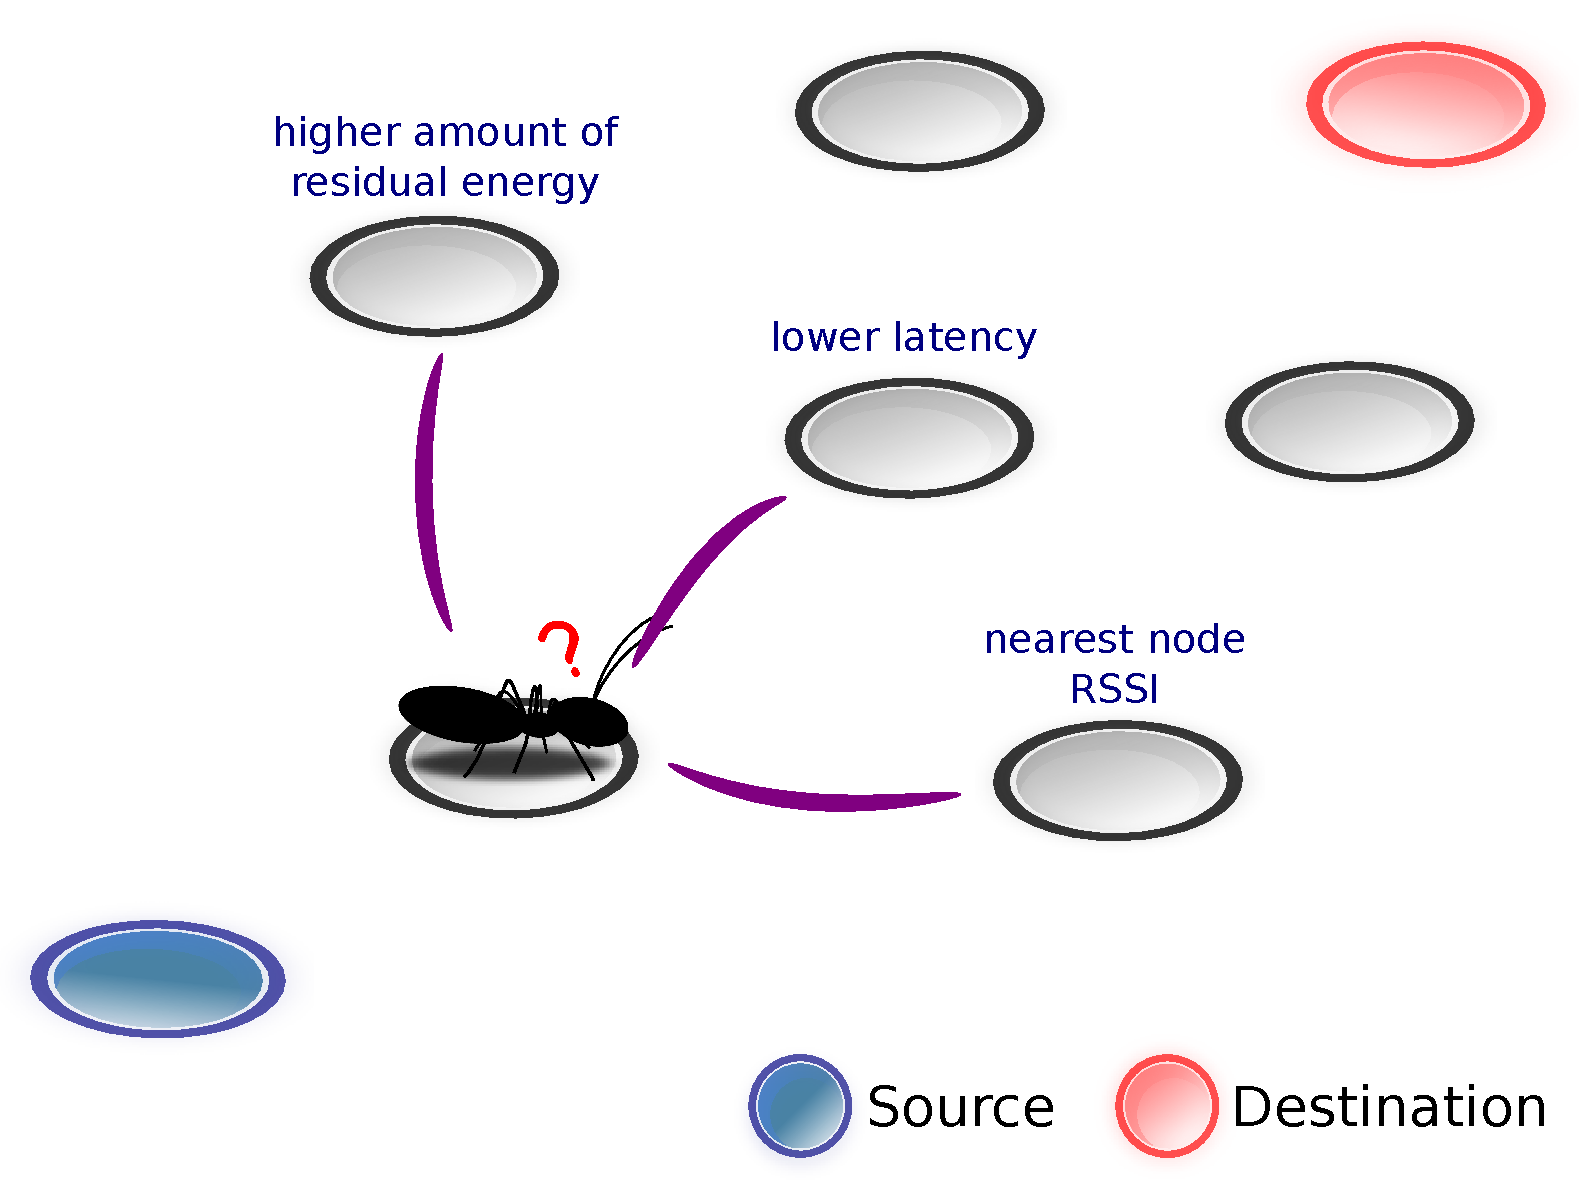
\includegraphics[width=220pt]{fig/ant_heuristic.pdf}
\caption{ADHOP heuristics}
\label{heuristics}
\end{figure}


\section{Performance Evaluation}
\label{evaluation}

In this performance evaluation, the implementations were performed using the OMNeT++ simulator.
It is an extensible, modular, component-based C++ simulation library and framework for building network simulators, and useful while modeling wireless communication.
The evaluation took place by way of a number of simulation scenarios using several routing protocols, such as AODV, DYMO, OLSR, DSDV, and ADHOP.

Table \ref{omnet} shows the OMNeT++ simulation parameters.
Similarly from the previous stage, each simulation scenario was run for a total of 300 seconds in an environment of high mobility that is conducive to high data loss.
Differently, such scenarios are more suitable for analysis of sensor networks.
The nodes are placed randomly in a rectangular area of 1000 meters x 1000 meters, and each one moves at a maximum speed of 5 meters per second, according to the Mass Mobility algorithm.
The data traffic is generated from 20 mobile source nodes to other 20 mobile sink nodes.
In the physical layer, the sensitivity is set to -85 dBm, the transmitter power is set to 1 mW, and the thermal noise is set to -110 dBm.
This base scenario was used for the experiments on OMNeT++.
The test scenarios are obtained by varying specific parameters in a base scenario, such as number of nodes.
The number of nodes ranged from 20 to 100.

\begin{table}[htbp]
\centering
\begin{tabular}{l|r}
\hline \hline
\multicolumn{2}{l}{\bf{Parameter}}  \\
\hline
Simulation Time             & $300 s$           \\
Number of Nodes             & $20 \sim 100$     \\
Area                        & $1000 m X 1000 m$ \\
App. Msg. Length            & $32 B$            \\
App. Msg. Frequence         & $2 s$             \\
UDP Header Length           & $8 B$             \\
IP Header Length            & $20 B$            \\
Netmask                     & $255.255.0.0$     \\
ADHOP Header Length         & $20 B$            \\
IEEE 802.15.4 ACK           & True              \\
IEEE 802.15.4 Header Length & $22 B$            \\
IEEE 802.15.4 Max Frame Size& $102 B$           \\
Phy. Transmitter Power      & $1 mW$            \\
Phy. Sensitivity            & $-85 dBm$         \\
Phy. Thermal Noise          & $-110 dBm$        \\
Channel Carrier Frequency   & $2.4 GHz$         \\
\hline
\end{tabular}
\caption{OMNeT++ Configuration}
\end{table}


Figure \ref{o_routing_overhead} shows the comparison between the protocols for routing overhead.
AODV and DYMO are reactive routing protocols which aim at producing less routing overhead.
However, in an environment that all nodes are constantly moving, a lot of data packets tend to be dropped.
These protocols have to maintain correct routes to their destinations thus increasing the routing overhead.
As mentioned earlier, AODV uses RQ, RP, and RE as messages to build and maintain routes.
Considering the high mobility and the high rate of data loss of the simulation performed, AODV tend to have a great load of control packets.
Each time a route breaks, AODV flood these messages within the network to notify and/or define a new route.
DYMO uses the same procedures.
Likewise, ADHOP is a reactive protocol, but it is also a protocol aware network flow.
It does not have repair procedures and only relies on pheromone, hence it does not produce any additional overhead.
We notice from the figure that ADHOP gives lower routing overhead due to a reduction of ants in the network.
Moreover, the data is sent along with the ants thereby decreasing the amount of control packets in the network.
Therefore, the routing overhead of our protocol tends to stay almost constant for large and dense networks.
OLSR and DSDV are proactive protocols; therefore, the overhead is expected to be high.
Regardless of what happens in the network, these routing protocols tend to maintain the overhead under control.
Because proactive protocols maintain their tables regularly updated thus the nodes do not tend to resort to repair procedures.

\begin{figure}[htbp]
\centering
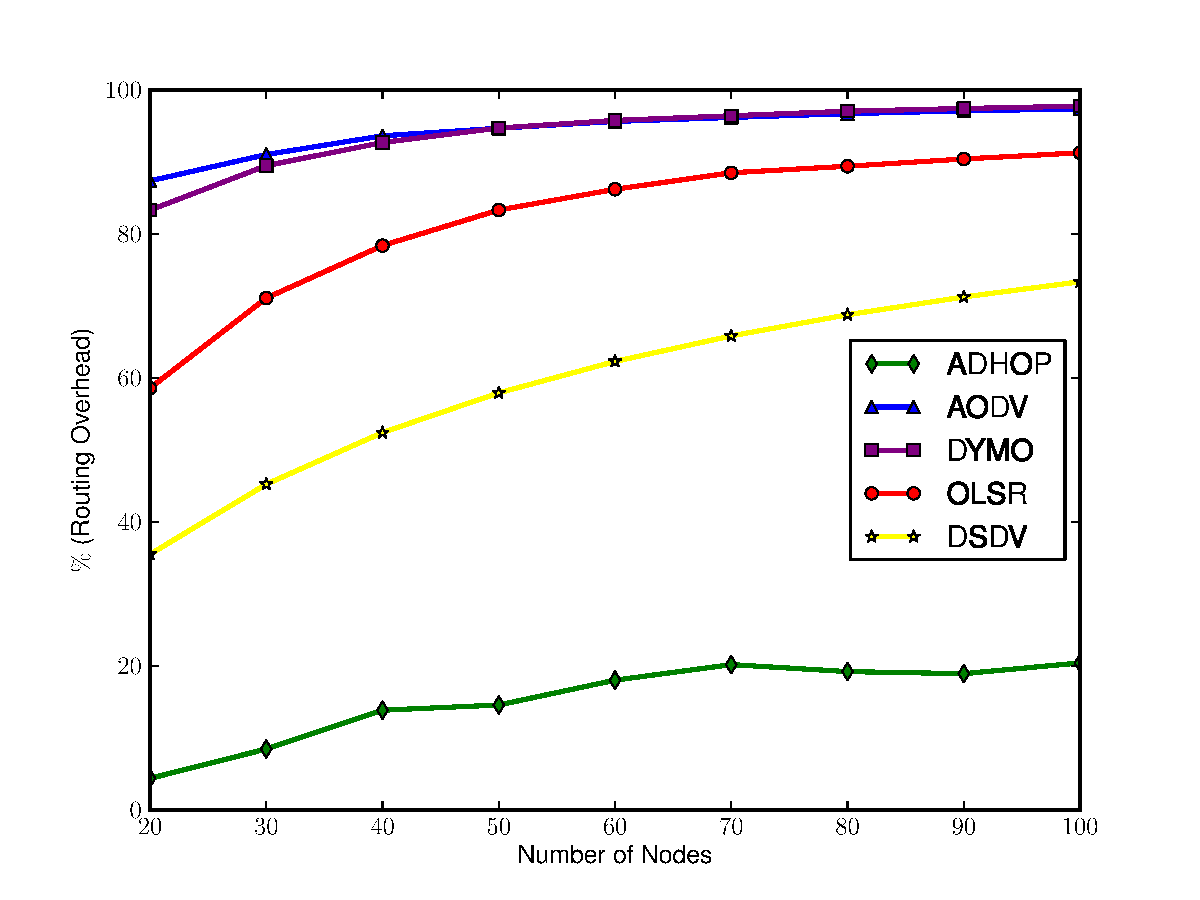
\includegraphics[width=250pt]{fig/o_routing_overhead.pdf}
\caption{Routing Overhead}
\label{o_routing_overhead}
\end{figure}

Figure \ref{o_link_failures} shows the results of dropped frame ratio due to link failures.
It is too hard to maintain IEEE 802.15.4 node's connectivity for mobile networks.
Moreover, the connectivity becomes worse with higher speeds and when all nodes are mobile \cite{Zen:2008}.
This low connectivity degrades the data delivery ratio due to the lack of synchronization with coordinators.
The low connectivity adds to the link failure ratio.
Especially in protocols such as ADHOP and DSDV that adapt to topology changes while producing low overhead in the network.
On the other hand, protocols such as OLSR that focus on the link state tend to have lower link failure ratio.
For this reason, we can notice that some routing protocols produces better results of link failures than ADHOP.
Similarly from the previous stage, our approach is a reactive routing protocol which uses only pheromone to make routing decisions.
Therefore, the links between neighbor nodes tend to be more susceptible to failure in order to adapt to topology changes.

\begin{figure}[htbp]
\centering
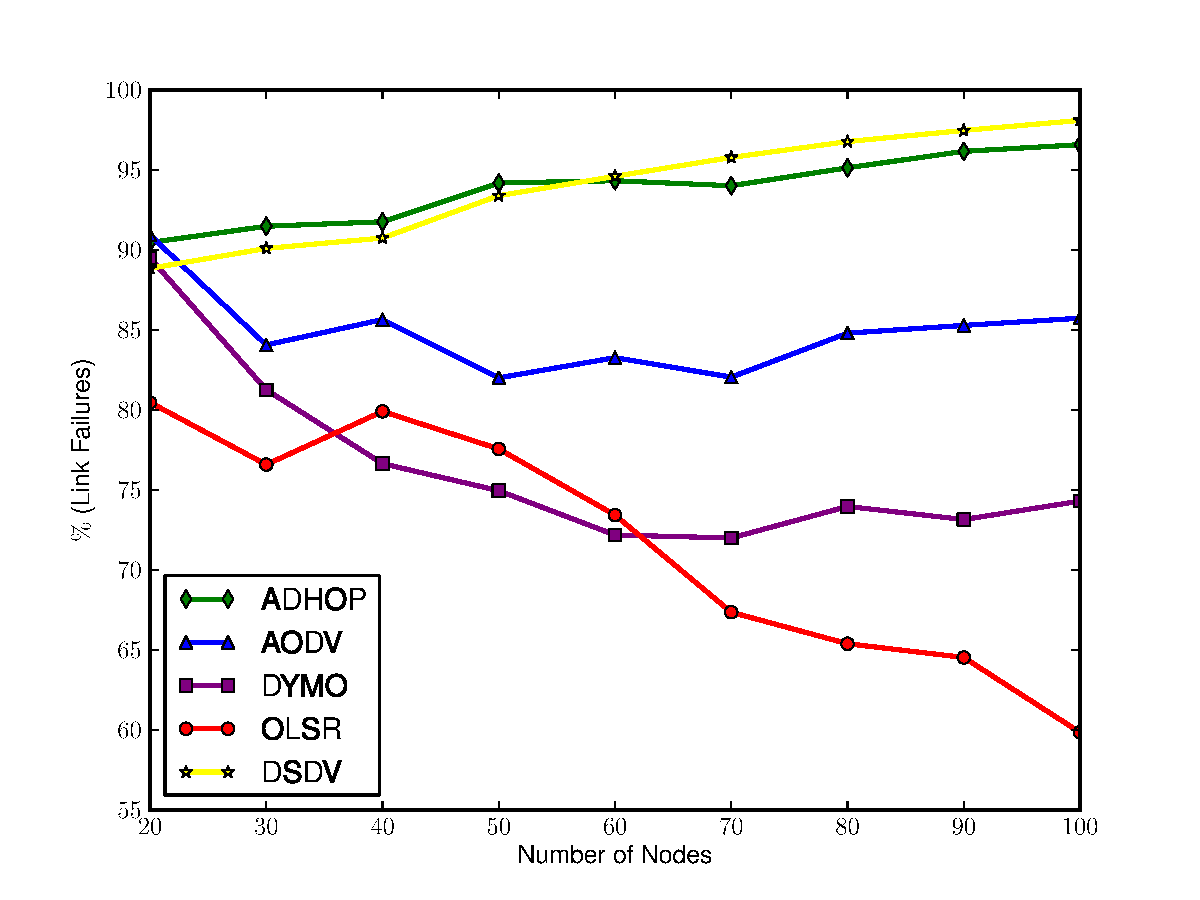
\includegraphics[width=250pt]{fig/o_link_failures.pdf}
\caption{Link Failures}
\label{o_link_failures}
\end{figure}

Figure \ref{o_broken_routes} shows the dropped frame ratio due to broken routes.
We notice that ADHOP and DSDV produce a lower rate of packet loss due to broken routes.
Both are protocols which tend to adapt to topology changes thus building the most reliable routes.
Differently, OLSR has difficulties in maintaining and disseminating the updated state of links in the form of routes at the time of data transmission.

\begin{figure}[htbp]
\centering
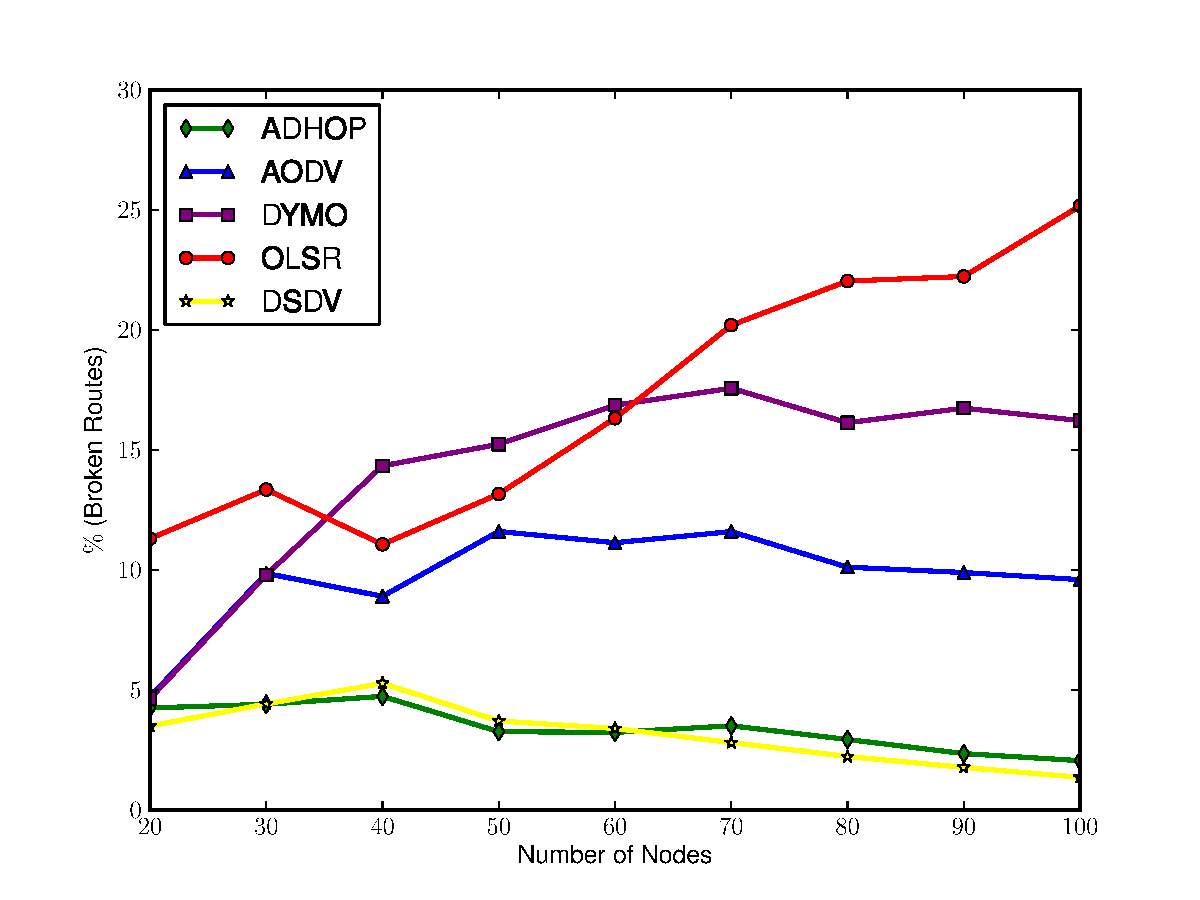
\includegraphics[width=250pt]{fig/o_broken_routes.pdf}
\caption{Broken Routes}
\label{o_broken_routes}
\end{figure}

Figure \ref{max_o_data_delivery_ratio} shows the maximum delivery ratio of AODV, DYMO, OLSR, and DSDV in this simulated IEEE 802.15.4 network.
This maximum delivery ratio does not consider the effects of packet loss due to broken routes.
Hence, by considering the effects of packet loss due to link failures, it is possible to calculate the maximum of packets transmitted successfully in a scenario which uses IEEE 802.15.4 standard.

\begin{figure}[htbp]
\centering
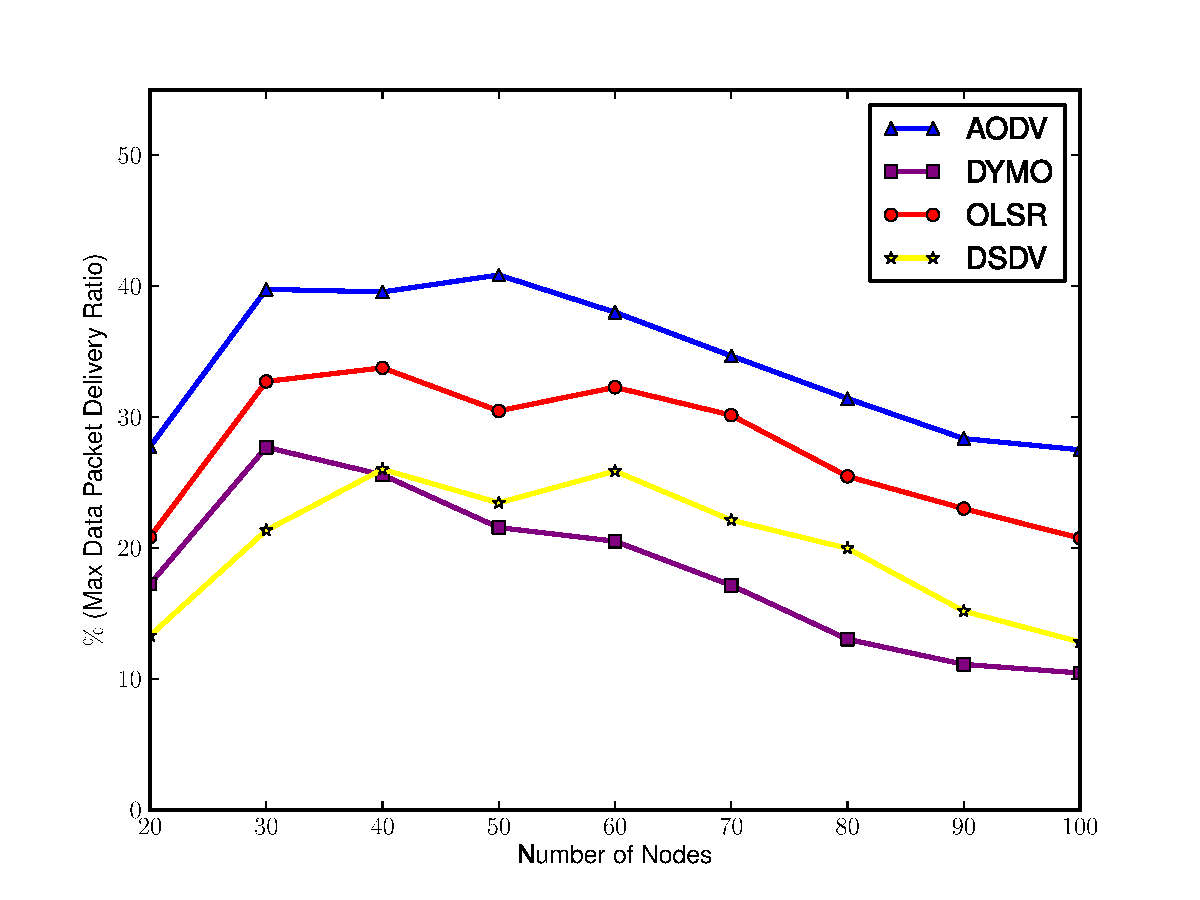
\includegraphics[width=250pt]{fig/max_o_data_delivery_ratio.pdf}
\caption{Maximum Data Packet Delivery Ratio}
\label{max_o_data_delivery_ratio}
\end{figure}

Figure \ref{o_data_delivery_ratio} shows the data packet delivery ratio in this simulation environment.
As an environment conducive to high data loss and high link failure ratio, the delivery ratio tends to decrease whilst the number of nodes and the routing overhead increases.
The minimization of protocol overhead may have to be the first course of action for WSNs with continuous changes in network topology.
ADHOP follows this concept thus affecting its data delivery ratio.
Moreover, as the number of node increases, the delivery ratio also increases due to the dynamic hop method which makes it able to direct the packets to a safer route.
If the network is too large and dense, then the delivery ratio is higher due to the large number of routes choices.
On the other hand, if the network is small and sparse, then the delivery ratio decreases due to lack of connectivity among nodes.
We notice from the figure that ADHOP shows better results of data delivery ratio for networks with high scalability and high mobility.

\begin{figure}[htbp]
\centering
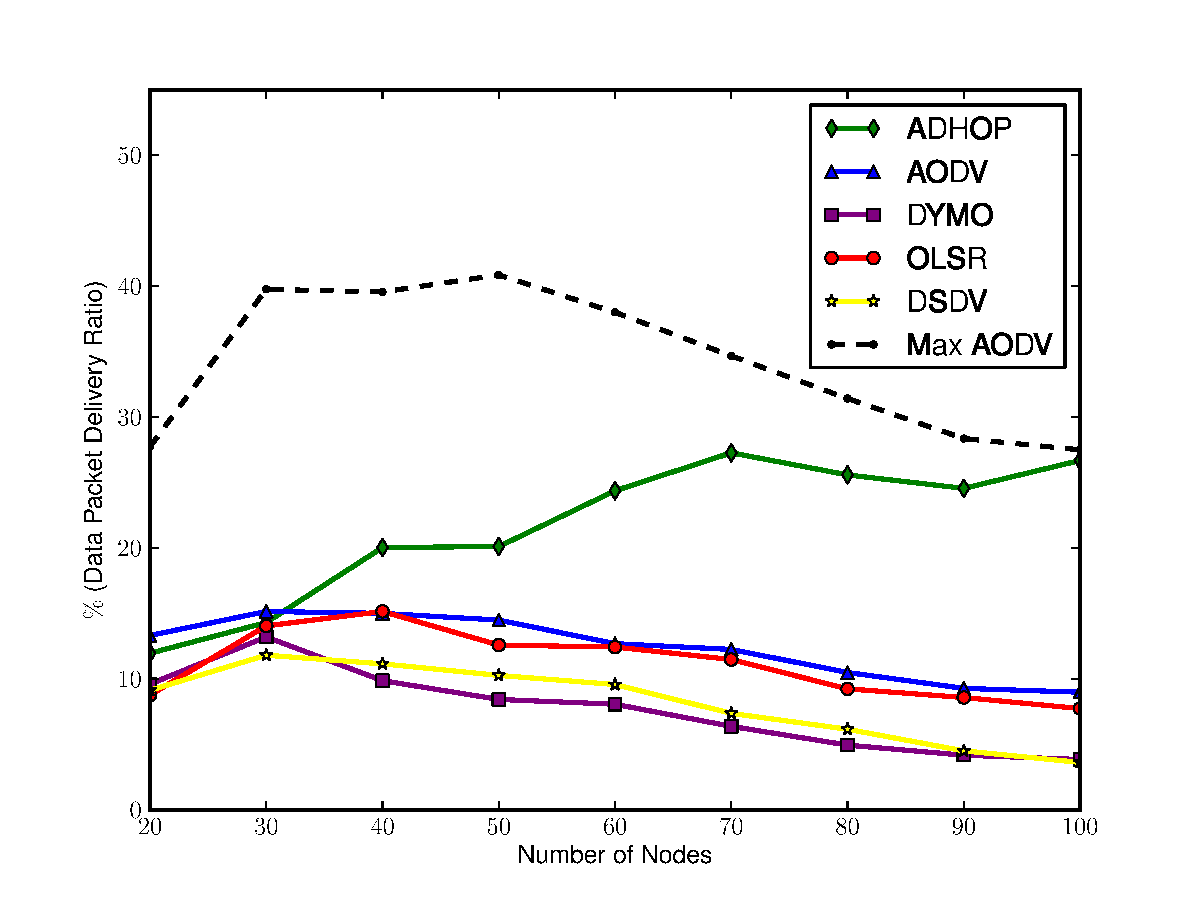
\includegraphics[width=250pt]{fig/o_data_delivery_ratio.pdf}
\caption{Data Packet Delivery Ratio}
\label{o_data_delivery_ratio}
\end{figure}

\section{Conclusion}
\label{conclusion}

In this paper, we introduce a new routing method based on dynamic hops and present ADHOP, a routing algorithm inspired on the ACO-based algorithms for mobile WSNs.
ADHOP uses pheromone as a metric to make routing decisions through the ACO meta-heuristic, and uses heuristic information for evaporation and pheromone deposit ratio.
We have evaluated and compared our algorithm to several routing for MANETs in a WSN environment and obtained better results in terms of data delivery ratio, routing overhead, and congestion avoidance for environments of dynamic topology.
We also conclude that in mobile networks, reactive routing protocols which are not aware of network flow make it worse than proactive protocols in terms of routing overhead.
Our proposal focuses primarily on routing overhead to reduce the amount of control packets in the network to require less effort in communication.
In fact, ADHOP achieves these results through the routing method based on dynamic hops which tends to keep the best routes in terms of connectivity without significant losses in the data delivery ratio.
Dynamic hops allow us to improve the routing and to avoid the necessity of complex structures and procedures thus increasing the efficiency and reducing the routing complexity for mobile WSNs.

\bibliographystyle{abbrv}
\bibliography{paper}

\end{document}

